\chapter{Common-Collector BJT Amplifier}


\section{Objectives}
\begin{itemize}
    \item To measure the quiescent-point of an emitter follower
    \item To evaluate the small-signal amplification function of an emitter follower
\end{itemize}

\section{Materials}
\begin{itemize}
    \item \hyperref[2N3904_1]{BJT (2N3904)}
    \item Breadboard
    \item Capacitors
    \item DC power supply
    \item Digital Multi-Meter
    \item Function Generator
    \item Oscilloscope
    \item Resistors
\end{itemize}

\section{Introduction}
    \subsection{Circuit Diagram}
    \begin{figure}[h]
        \centering
        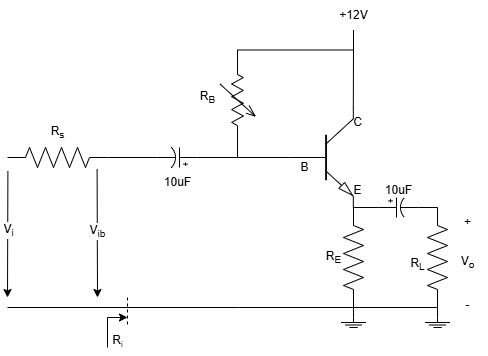
\includegraphics[width=0.7\linewidth]{Lab07/Lab7.drawio.png}
        \caption{A common-collector BJT amplifier/emitter follower.}
        \label{l7f}
    \end{figure}
    \FloatBarrier
In Fig.\ref{l7f}, $V_{BEQ}$ = 0.6 V, $\beta$ = 160, $R_s$ = 10k$\Omega$, $R_B$ = 56k$\Omega$, $R_E$ = 1k$\Omega$.

\section{Detailed Procedures}
    \subsection{Analyzation}
    First, we analyze the circuit by drawing its AC-equivalent and DC-equivalent circuit.\par
    \begin{itemize}
        \item AC-equivalent Circuit:\par
            \begin{figure}[h]
                \centering
                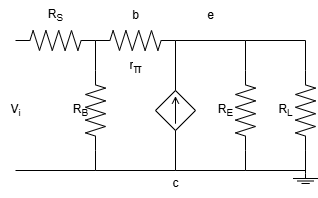
\includegraphics[width=0.65\linewidth]{Lab07/Lab7ac.drawio.png}
                \caption{AC-equivalent Circuit}
                \label{l7ac}
            \end{figure}
            \FloatBarrier
        \item DC-equivalent Circuit:\par
            \begin{figure}[h]
                \centering
                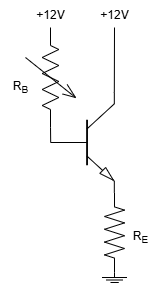
\includegraphics[width=0.3\linewidth]{Lab07/Lab7dc.drawio.png}
                \caption{DC-equivalent Circuit}
                \label{l7dc}
            \end{figure}
            \FloatBarrier
    \end{itemize}
    \FloatBarrier
    To analysis Fig.\ref{l7ac} and Fig.\ref{l7dc} with given data, we can obtain:\par
    In Fig.\ref{l7ac}\par
    \begin{equation}
        \begin{cases}
            R_{TH} = R_a//R_b\\
            V_{TH} = 12\cdot\frac{R_b}{R_a//R_b}\\
            12-i_cR_c-V_{CE}-i_ER_E=0\\
            V_{TH}-i_bR_{TH}-V_{BE}-i_eR_E=0\\
        \end{cases}
    \end{equation}
    
    In Fig.\ref{l7dc}\par
    \begin{equation}
        \begin{cases}
            A_v = \frac{V_i}{V_o} = \frac{I_B(1+\beta)(R_E//R_L)}{r_\pi+(1+\beta)(R_E//R_L)}\frac{R_i}{R_i+R_S}\\
            R_i = R_B\\
            R_o = R_E//R_L\\
        \end{cases}
    \label{l7eq1}
    \end{equation}

    \subsubsection{DC Analysis}
    \begin{equation*}
        \begin{cases}
            I_{BQ}=52.53\mu A\\
            I_{EQ}=8.4573mA\\
            I_{CQ}=8.4048mA\\
            V_B=9.0583V\\
            V_C=12V\\
            V_E=8.4581V\\
            V_{CEQ}=3.5419V\\
        \end{cases}
    \end{equation*}
    \FloatBarrier
    
    \subsection{Procedures}
    Construct the circuit in Fig.\ref{l7f} with an npn BJT and $R_L$ = 300k$\Omega$.
        \subsubsection{DC Analysis}
        Short $v_i$ to the ground and use the digital multi-meter to measure the three terminal voltages of the BJT $V_B$, $V_C$, and $V_E$:\\
            \begin{equation}
                \begin{cases}
                    V_B=10.10\\
                    V_C=12\\
                    V_E=9.505\\
                \end{cases}
            \label{L7Eq1}
            \end{equation}
            From Eq.\ref{L7Eq1}, we can obtain:\\
            \begin{equation}
                \begin{cases}
                    I_{BQ}=\frac{V_C-V_B}{R_B}=33.929\mu A\\
                    I_{EQ}=\frac{V_E}{R_E}=9.505mA\\
                    I_{CQ}=I_{EQ}-I_{BQ}=9.471mA\\
                    \beta=279.14\\
                \end{cases}
            \end{equation}
        The experimental data differs from theoretical calculation with all data is reduced. It might be caused by unideal power supplied or unideal resistors.

        \subsubsection{AC Analysis}
        \begin{itemize}
            \item Voltage Gain: Let $v_i$ to be a sinusoidal signal (1000 Hz, 5V peak) and $R_L$ = 300k$\Omega$.
                \begin{table}[h]
                \centering
                \begin{tabular}{|c|c|c|c|c|}
                    \hline
                    Vib & 0.9372     & 0.7239      & 0.4901    & 0.24     \\ \hline
                    Vo  & 0.9425     & 0.7072      & 0.4824    & 0.2411   \\ \hline
                    Av  & 1.00565514 & 0.976930515 & 0.9842889 & 1.004583 \\ \hline
                \end{tabular}
                \end{table}
                \FloatBarrier
                When the BJT turns to saturation, the distortion occurs. $R_B$ should be increased to enlarge the linear amplification range.
            \item Input \& Output Resistance: Let $v_i$ to be  a 1000 Hz sinusoidal signal with the amplitude of 1 V.
                \begin{table}[h]
                \centering
                \begin{tabular}{|cc|cc|}
                    \hline
                    \multicolumn{2}{|c|}{Rs=10K,Ri=10.3K}     & \multicolumn{2}{c|}{Ro=36.4}                             \\ \hline
                    \multicolumn{1}{|c|}{Vi=1.15} & Vib=0.578 & \multicolumn{1}{c|}{RL=300K,Vo=0.5883} & RL=1K,Vo=0.5683 \\ \hline
                \end{tabular}
                \end{table}
                \FloatBarrier
        \end{itemize}
        
    
\section{Discussion}
    Some measured data are missing due to inappropriate saving in this experiment report. Using other groups data instead.

\section{Conclusion}
    In this experiment, we implemented the common-collector BJT amplifier circuit. This experiment deepen our understanding of BJT circuit, the common-collector circuit is characterized by the connection of the base and collector through a resistor. By analyzing the amplifier's performance through oscilloscope, we learn about the role of biasing, the effects of input and load resistance.\par
    Overall, this experiment provided valuable practical considerations for designing amplifiers in real-world applications, particularly in minimizing signal distortion and optimizing performance.